\documentclass[UTF8, xcolor=table]{beamer}
\usepackage[BoldFont,SlantFont]{xeCJK}
\setCJKmainfont[Extension=.otf,BoldFont=FandolHei-Regular,ItalicFont=FandolKai-Regular]{FandolSong-Regular}
%\setCJKmainfont[BoldFont={Adobe Heiti Std},ItalicFont={Adobe Kaiti Std}]{SimSum} %Windows先编译使用这个字体

\usepackage{latexsym,amssymb,amsmath,amsbsy,amsopn,amstext,xcolor,multicol}
\usepackage{graphicx,wrapfig,fancybox}
\usepackage{pgf,pgfarrows,pgfnodes,pgfautomata,pgfheaps,pgfshade}
\usepackage{thubeamer}
\usepackage[backend=bibtex,sorting=none]{biblatex} % [参考文献格式](https://www.sharelatex.com/blog/2013/07/31/getting-started-with-biblatex.html) %mac IEEE not found
\usepackage{array}
\usepackage{bm}
\usepackage{caption}
\RequirePackage[font=footnotesize]{subcaption}
\usepackage{multirow}
\usepackage{booktabs}
\usepackage{tikz}
\usepackage{tikzscale}
\usepackage{animate}

\defbibheading{bibliography}[\bibname]{} %avoid printbibliography 自动生成目录
\addbibresource{../main.bib}
\setbeamertemplate{bibliography item}[text] 

\usepackage{boxedminipage} %for: bvh border
\def\fourgraphicswidth{0.35} %0.3\textwidth

\usepackage{algorithm} %%format of the algorithm
\usepackage{algpseudocode}
\floatname{algorithm}{算法}
\renewcommand{\algorithmicrequire}{\textbf{输入:}} % Use Input in the format of Algorithm
\renewcommand{\algorithmicensure}{\textbf{输出:}} % UseOutput in the format of Algorithm
\algrenewcommand{\algorithmiccomment}[1]{ $//$ #1}

\usepackage{listings}
\renewcommand\lstlistingname{代码}
\renewcommand\lstlistlistingname{代码}

\lstset{framexleftmargin=1.4em,
        xleftmargin=1.8em,
        basicstyle=\ttfamily\small,
        %frame=shadowbox, numberstyle=\tiny, breaklines=true,
        frame=single,
        numberstyle=\tiny, breaklines=true,
        keywordstyle=\color{blue!70}\bfseries,
        %commentstyle=\color{red!50!green!50!blue!50},
        rulesepcolor=\color{red!20!green!20!blue!20},
        numbers=none,fontadjust=true}
\lstdefinelanguage{shader}{morekeywords={uniform, layout, uniform, vec2, vec3, vec4, in, out, gl_Position, dot, flat, int ,float, gl_VertexID, xyz, w, x, y, z, location, version, sampler2DRect, bgr, gl_FragData, texture2DRect, gl_TexCoord,for,xy},morecomment=[l]{//}}

\begin{document}

\setbeamerfont{footnote}{size=\tiny}
\setbeamerfont{caption}{size=\scriptsize}
\setbeamertemplate{caption}[numbered]
\setbeamerfont{subsection in toc}{size=\footnotesize}
\renewcommand*{\bibfont}{\footnotesize}

\graphicspath{{../}}

\title[融合长短记忆神经网络与卷积特征学习的图像语义分割]{中山大学本科毕业论文演示文稿非正式模版}
\author[陈冠英]{}%{(申请中山大学工学学士学位论文答辩报告)\\ \vskip 20pt 学~~~~~~生:陈~冠~英}
\institute[中山大学~电子信息与工程学院~\&~自动化]{}%{\small \vskip 38pt 电子信息与工程学院~自动化}
\date{} %{\small \vskip -17pt二〇一六年五月}

%% make title %%
\frame{
	\titlepage
	\vspace{-23mm}
	\begin{figure}[h]
		\centering
		\includegraphics[width=\textwidth]{image/illustration/networkstructure.pdf}
	\end{figure}
}

\frame {
	\frametitle{目录}
	%\begin{multicols}{2}
	\tableofcontents[sections={<1-7>}]
}

%%
% 引言或背景
% 引言是论文正文的开端,应包括毕业论文选题的背景、目的和意义;对国内外研究现状和相关领域中已有的研究成果的简要评述;介绍本项研究工作研究设想、研究方法或实验设计、理论依据或实验基础;涉及范围和预期结果等。要求言简意赅,注意不要与摘要雷同或成为摘要的注解。
%%
% 章、节、小节、图片、公式、表格下方的\label{...}标记不建议删除,因为这些可以做到自动引用的作用,当某些公式、图片被删除时,\label{...}标记能使正文中的编号自动更新,省去一个一个编号的麻烦。

\chapter{绪论}
\label{cha:introduction}
\section{引言}
\label{sec:prologue}
引言是论文正文的开端,应包括毕业论文选题的背景、目的和意义;对国内外研究现状和相关领域中已有的研究成果的简要评述;介绍本项研究工作研究设想、研究方法或实验设计、理论依据或实验基础;涉及范围和预期结果等。要求言简意赅,注意不要与摘要雷同或成为摘要的注解。

\section{国内外研究现状和相关工作}
\label{sec:related_work}
对国内外研究现状和相关领域中已有的研究成果的简要评述。

\section{本文的论文结构与章节安排}
\label{sec:arrangement}
本文共分为五章,各章节内容安排如下:

第一章引言。

第二章知识点。

第三章方法介绍。

第四章实验和结果。

第五章是本文的最后一章,总结与展望。是对本文内容的整体性总结以及对未来工作的展望。


\chapter{本模板的一些基本设定}
\label{cha:format}
本章将介绍本模板的一些基本设定。
\section{版面}
\label{sec:composition}
在介绍本模板的排版和格式之前,本章首先介绍一些基本的概念,如图 \ref{fig:composition_general} 所示。图 \ref{fig:composition_general} 中的英文为geometry宏包中的参数,纸张默认设置为A4大小,body或total body为正文内容所在区域。重要的参数有7个,分别是:top、bottom、left、right、headheight、headsep、footskip。top和bottom分别为上边距和下边距,本模板按照word默认设置为1英寸;left和right分别为左边距和右边距,本模板设置为1英寸;headsep为页眉(横线)与正文区域的距离,本模板按照word默认设置为0.2英寸;headheight为页眉内容的高度,本模板按照word默认设置页眉顶端距离页面边界1.5 cm,计算得到headheight为0.532 cm;footskip为页脚内容的高度,本模板按照word默认设置页脚底部距离页面边界1.75 cm,计算得到footskip为0.79 cm。
\begin{figure}[H] 
	\centering
	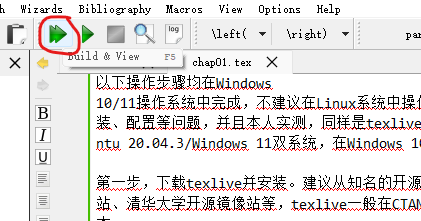
\includegraphics[width=0.6\textwidth]{image/chap01/f5.png}
	\caption{Build \& View}
	\label{fig:f5}
\end{figure}

每一章的标题采用小二号黑体,居中;节标题采用小三号宋体,加粗;小节标题采用小四号宋体,加粗(本模板中,由于选用的字库和字体问题,无法直接将宋体加粗,于是实际采用黑体代替宋体加粗)。正文内容、致谢和附录中的中文采用小四号宋体,英文采用Times New Roman,12 pt。参考文献的字体和字号采用宋体/Times New Roman,五号/10 pt。行距设置为1.5倍行距。



\chapter{图像的插入示例}
\label{cha:fig_example}
除了第一章引言和最后一章的总结与展望之外,正文的所有章都要在章标题之下加上这样一段引入本章内容的话语,让读者知道本章的目的以及意义。本章将通过一些示例来说明如何插入图片。读者在阅读文章时,最能吸引读者注意力的莫过于文章中的图片,因此图片对于论文来说是重中之重,甚至可以说,好图就是好文章。规范地插入图片对于整篇文章的观感、阅读体验来说,有着至关重要的作用。
\section{单张图片的插入}
\label{sec:fig_singlefig}
单张图片插入的原则:(1)图片居中放置,大小适当,图中文字、内容清晰;(2)从文献中获得的图片要引用,要写明来源;(3)图片应该放置在两段文字之间,图片上面一段文字应该是对图片内容的描述,不要插在一段文字内,一页排不下时,应排在下一页的顶部;(4)对图片的描述要符合规范,指明是图x-x,不能说如下图所示。

错误描述:托卡马克装置示意图如下图所示\cite{xu2016general}:

正确描述:托卡马克装置示意图如图 \ref{fig:tokamak} 所示\cite{xu2016general}:
\begin{figure}[htbp] % 图片排序优先级,h表示当前位置,t表示顶部,b表示底部,p表示浮动页,可以是单独一个字母或者几个字母的组合
	% 居中
	\centering
	% 图片宽度、图片文件名及在硬盘中的位置
	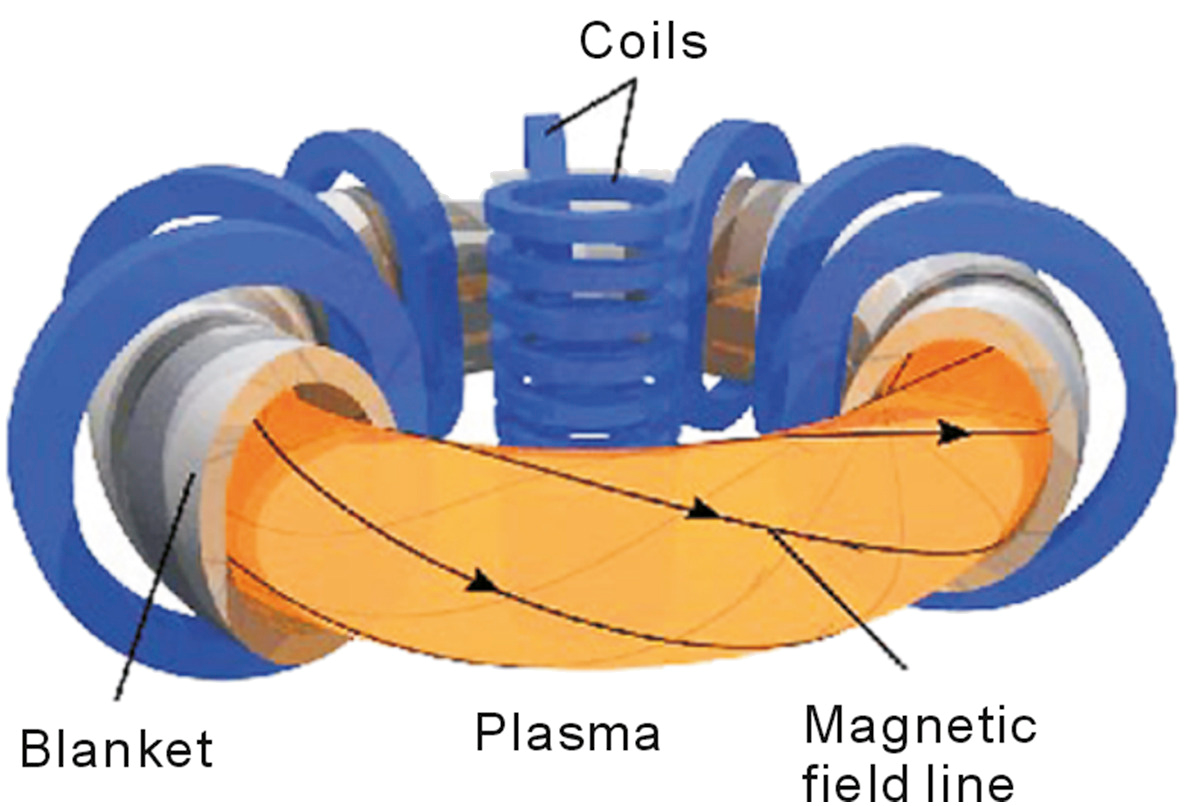
\includegraphics[width=0.6\textwidth]{image/chap03/tokamak.png}
	% 图片下标题
	\caption{托卡马克装置示意图\cite{xu2016general}}
	% 图片标签
	\label{fig:tokamak}
\end{figure}
\subsection{矢量图片的插入}
\label{ssec:fig_vecfig}
本小节示例了如何插入小节。按照中大的规定,正文中的标题只到小节,如 \ref{ssec:fig_vecfig} 小节,目录中的标题只到节,如 \ref{sec:fig_singlefig} 节。

\LaTeX\  支持svg、pdf、eps格式的矢量图的插入,svg格式的矢量图插入过程有点复杂,我暂时还没看明白,但是pdf和eps格式的矢量图是能直接插入的,操作很简单,与图 \ref{fig:tokamak} 操作相同,只需更改文件名。

图 \ref{fig:tbm_layer} 为插入的pdf格式的矢量图,图 \ref{fig:confusion} 为插入的eps格式的矢量图。一些简单的示意图可以用PowerPoint制作,最后导出成pdf即可,值得注意的是,MS Office套件由于自身的漏洞,无法导出eps格式的文件。
\begin{figure}[H] % H表示强制图片位置,配合float宏包使用,模板中已配置
	\centering
	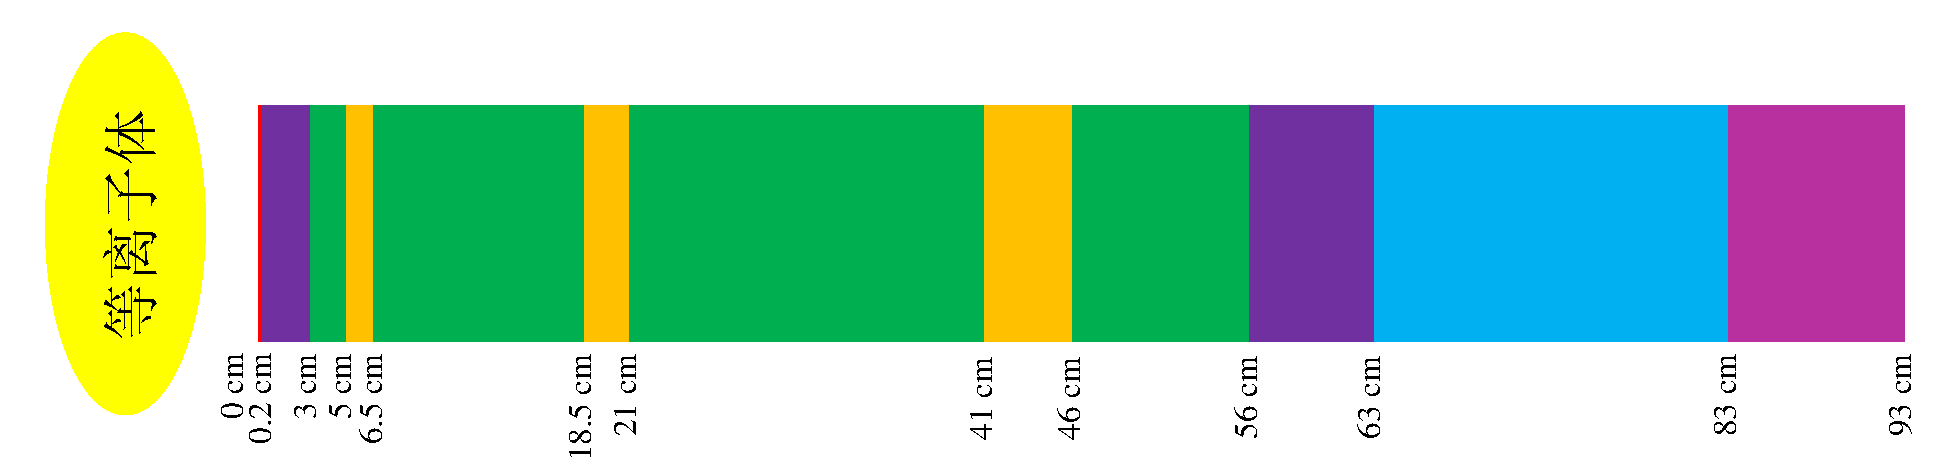
\includegraphics[width=1\textwidth]{image/chap03/tbm_layer.pdf}
	\caption{插入的pdf格式矢量图}
	\label{fig:tbm_layer}
\end{figure}
\begin{figure}[h]
	\centering
	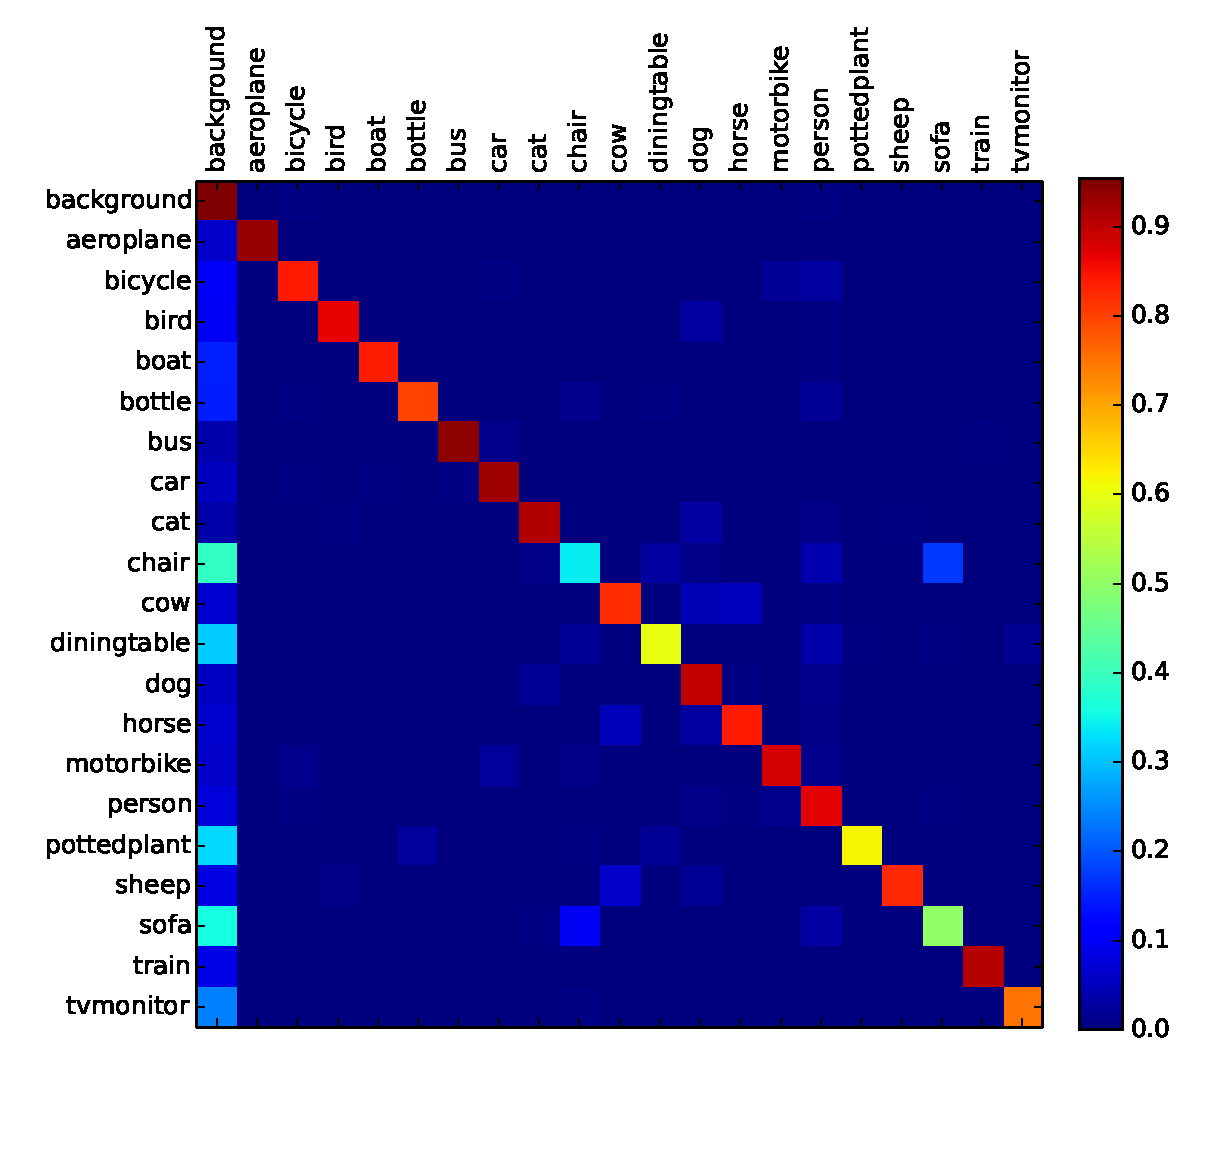
\includegraphics[width=0.6\textwidth]{image/chap03/confusion.eps}
	\caption{插入的eps格式矢量图}
	\label{fig:confusion}
\end{figure}
\section{多张图片的插入}
\label{sec:fig_multifig}
多张图片插入的原则与单张图片的相同,但是值得注意的是,多张图片不宜使用\LaTeX\ 直接插入,应将所需插入的图片先用PowerPoint排列、拼接,再标号,生成一张图片,再整个插入论文中,这样就与单张图片的插入过程相同。生成图片的过程,偷懒的话可以直接截屏保存为png格式图片,不偷懒就调整ppt的大小后直接导出为pdf。
\begin{figure}[h] 
	\centering
		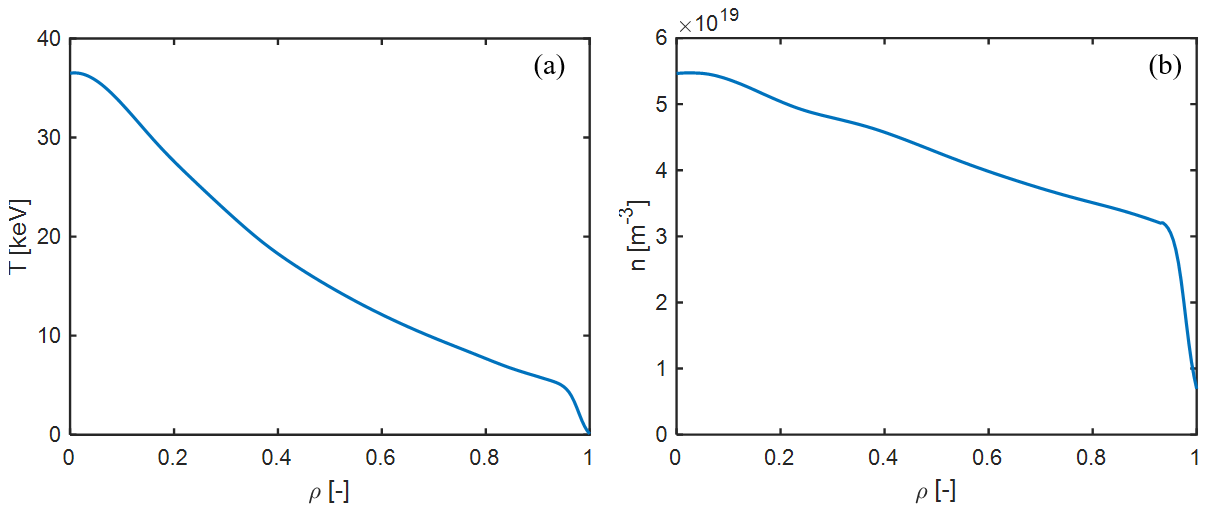
\includegraphics[width=1\textwidth]{image/chap03/temperature_density.png}
		\caption{简单的两张图片插入。(a)温度分布;(b)密度分布}
		\label{fig:temperature_density}
\end{figure}
\begin{figure}[h]
	\centering
	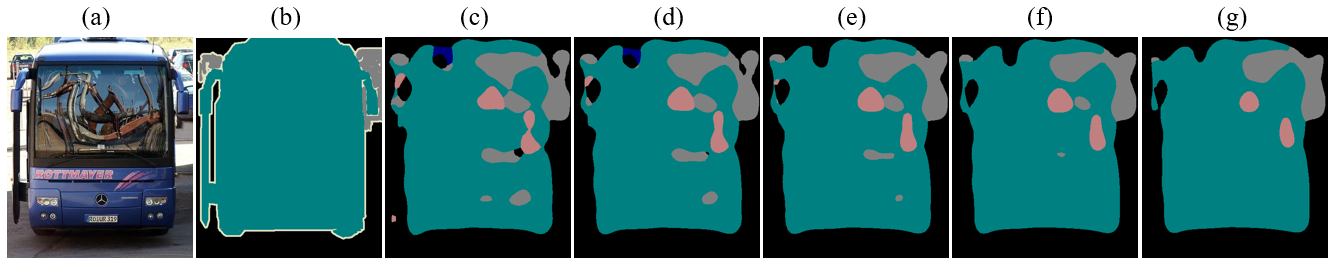
\includegraphics[width=1\textwidth]{image/chap03/compare.png}
	\caption{多张图片并排插入。(a)图像;(b)真值;(c) CNN+5LSTM1;(d) CNN+5LSTM2;\\ (e) CNN+5LSTM3;(f) CNN+5LSTM4;(g) CNN+5LSTM5}
	\label{fig:compare}
\end{figure}

\section{本章小结}

\chapter{公式与表格的插入示例}
\label{cha:for_tab_example}
公式用于对论文基础理论的介绍,表格则是对一些不方便进行作图的数据进行展示。

\section{公式的插入}
\label{sec:formula}
带左半边大括号的核反应方程式,如式(\ref{eqn:fusion_reactions})所示:
\begin{equation}
	\label{eqn:fusion_reactions}
	\left\{
	\begin{aligned}
		&\mbox{D}+\mbox{D}\rightarrow \mbox{T}\,(\text{1.01}\;\mbox{MeV})+\mbox{p}\,(\text{3.03}\;\mbox{MeV}) \\
		&\mbox{D}+\mbox{D}\rightarrow {^{\text{3}}}\mbox{He}\,(\text{0.82}\;\mbox{MeV})+\mbox{n}\,(\text{2.45}\;\mbox{MeV}) \\
		&\mbox{D}+\mbox{T}\rightarrow \text{α}\,(\text{3.52}\;\mbox{MeV})+\mbox{n}\,(\text{14.06}\;\mbox{MeV}) \\
		&\mbox{D}+{^{\text{3}}}\mbox{He}\rightarrow \text{α}\,(\text{3.67}\;\mbox{MeV})+\mbox{p}\,(\text{14.67}\;\mbox{MeV})
	\end{aligned}
	\right.
\end{equation}

狄拉克函数$\delta_{ij}$的表达式:
\begin{equation}
	\label{eqn:delta_ij}
	\delta_{ij}=\left\{
	\begin{aligned}
		1&    &\mbox{if}&    &i=j \\
		0&    &\mbox{if}&    &i\neq j
	\end{aligned}
	\right.
\end{equation}

一般的公式:
\begin{equation}
	\label{eqn:vec_v_cm}
	\vec{v}_{cm}=\dfrac{m_{1}\vec{v}_{1}+m_{2}\vec{v}_{2}}{m_{1}+m_{2}}
\end{equation}

超长的公式:
\begin{equation}
	\label{eqn:iint_theta3_phi3}
	\begin{split}
		\int_{0}^{\pi}\int_{0}^{2\pi} \sin\theta_{3}&\dfrac{\exp(-\alpha v_{cm}^{2})}{v_{cm}}\sinh(\mu \gamma v_{r}v_{cm})\mbox{d}\phi_{3}\mbox{d}\theta_{3}=\dfrac{2\pi \sqrt{\pi}}{4\sqrt{\alpha}v_{3}u_{3}}\exp\left( \dfrac{(\mu \gamma v_{r})^{2}}{4\alpha} \right) \\
		&\times \Bigg( \mbox{erf}\left( \dfrac{\mu \gamma v_{r}+2\alpha(v_{3}-u_{3})}{2\sqrt{\alpha}} \right)-\mbox{erf}\left( \dfrac{-\mu \gamma v_{r}+2\alpha(v_{3}-u_{3})}{2\sqrt{\alpha}} \right) \\
		&+\mbox{erf}\left( \dfrac{-\mu \gamma v_{r}+2\alpha(v_{3}+u_{3})}{2\sqrt{\alpha}} \right)-\mbox{erf}\left( \dfrac{\mu \gamma v_{r}+2\alpha(v_{3}+u_{3})}{2\sqrt{\alpha}} \right) \Bigg)
	\end{split}
\end{equation}

输入矩阵:
\begin{equation}
	\label{eqn:matrix}
	\textbf{H} = \begin{bmatrix}
		I*\mybold{x}_i \\ \textbf{h}
	\end{bmatrix}
\end{equation}
\chapter{结论与展望}
\label{cha:conclusion_outlook}
% 第六章,有需要可自行使用

\end{document}
